
\documentclass{article}
\usepackage{graphicx} % Required for inserting images
\usepackage{fancyhdr} % Required for header and footer configuration
\usepackage[a4paper, margin=2.5cm, left=1.5cm, right=1.5cm, bottom=4cm]{geometry} % Required for setting page margins
\usepackage[T1]{fontenc}
\usepackage[default,oldstyle,scale=1]{opensans} % Utilizzo del font Open Sans
\usepackage{lipsum}
\usepackage{makeidx}
\usepackage{booktabs}
\usepackage{tabularray}
\usepackage[colorlinks=true, linkcolor=black, urlcolor=blue, citecolor=blue]{hyperref}
\usepackage{tabularx}
\usepackage{makecell}
\usepackage{enumitem} % Pacchetto per la personalizzazione degli elenchi
\usepackage{booktabs}
\usepackage{subcaption}

% Configure header and footer for the first page
\fancypagestyle{firstpage}{
    \fancyhf{} % Clear header and footer
    \renewcommand{\headrulewidth}{0pt} % Remove header rule line
    \lhead{} % Header on the left
    \chead{} % Header in the center
    \rhead{} % Header on the right
    \lfoot{} % Footer on the left
    \cfoot{\vspace{5pt}\\\hrulefill\\\vspace{10pt}\textbf{BeeLive}\\Gruppo 21} % Footer in the center
    \rfoot{\vspace{32.5pt}\\\thepage} % Footer on the right
}

% Configure header and footer for non-plain pages (second page onwards)
\fancypagestyle{nonplain}{
    \fancyhf{} % Clear header and footer
    \lhead{} % Header on the left
    \chead{} % Header in the center
    \rhead{
\includegraphics[width=2cm]{Images/BeeLive-Logo.png}\\\vspace{2pt}} % Header on the right
    \lfoot{} % Footer on the left
    \cfoot{\vspace{5pt}\\\hrulefill\\\vspace{10pt}\textbf{BeeLive}\\Gruppo 21} % Footer in the center
    \rfoot{\vspace{32.5pt}\\\thepage} % Footer on the right
}

% Adjust vertical space between header and text                                    
\setlength{\headsep}{65pt} 
% Adjust vertical space between text and footer
\setlength{\footskip}{0pt} 

\title{
\includegraphics[width=0.75\textwidth]{Images/BeeLive-Logo.png}\\\vspace{100pt}
\LARGE{\textbf{BeeLive\\Deliverable 2}}}
\author{Gruppo 21:\\
Cipriani Pietro, 226959\\
Orlando Dennis, 227688\\
Ziviani Elia, 228172}
\date{22 Aprile 2024}

\makeindex % Indica che vogliamo creare un indice

\begin{document}

\maketitle
\thispagestyle{firstpage} % Apply firstpage style to the first page
\clearpage

\pagestyle{nonplain} % Apply non-plain style to subsequent pages

\renewcommand{\contentsname}{Indice}
\tableofcontents

\clearpage

\section{Component Diagram}
\index{Component Diagram}

Questo capitolo è incentrato sull'analisi dei componenti del sistema che saranno realizzati.\\
Lo scopo è quello di descrivere ogni singolo componente in termini di funzionalità e interfacce.\\

I componenti sono individuati seguendo quando espresso nel documento Deliverable 1 per quanto riguarda i casi d'uso e sono definiti come entità autonome nel sistema.\\
Questi componenti sono provvisti di interfacce che permettono la comunicazione tra di essi.\\
Le interfacce sono definite come:
\begin{itemize}
    \item \textbf{Interfacce di OUTPUT}: Tutte quelle interfacce che offrono servizi al sistema.
    \item \textbf{Interfacce di INPUT}: Tutte quelle interfacce che ricevono servizi dal sistema.
\end{itemize} 

\subsection{Gestione utente}
\index{Gestione utente}

\begin{table}[htbp]
    \centering
    \begin{tabularx}{\textwidth}{| l | l | X |}
        \Xhline{2pt}
        \textbf{INPUT} & \textbf{Nome} & \textbf{Descrizione} \\
        \Xhline{2pt}
         & Notifiche & Il componente utilizza l'interfaccia fornita dal componente "Gestione Notifiche" per ricevere notifiche relative alle criticita' \\
        \hline
         & Auth & Il componente utilizza l'interfaccia fornita dal componente "Gestione Autenticazione" per richiedere il token necessario per effettuare il login \\
        \hline
         & Data & Il componente utilizza l'interfaccia fornita dal componente di gestione del database per scambiare tutti i dati necessari a garantire un corretto funzionamento dell'applicativo per gli utenti \\
        \hline
         & Percorsi &  \\
        \Xhline{2pt}
        \textbf{OUTPUT} & \textbf{Nome} & \textbf{Descrizione} \\
        \Xhline{2pt}
         & Login & Il componente fornisce un'interfaccia per effettuare il login attraverso i servizi del componente esterno CasDoor, che prevede l'inserimento delle specifiche credenziali per generare un token di accesso \\
        \hline
         & Logout & Il componente fornisce all'utente un'interfaccia per effettuare il logout \\
        \hline
         & Registrazione & Il componente fornisce all'utente un'interfaccia per registrarsi attraverso il servizio CasDoor \\
        \hline
         & Selezione aree & Il componente fornisce un'interfaccia che permette all'utente di specificare sulla mappa della citta' di Trento la sua zona di maggior interesse per poi considerare quella zona come utile per la visualizzazione dei dati \\
        \hline
         & Visualizzazione evento & Il componente fornisce un'interfaccia che permette la visualizzazione di tutti gli eventi presenti sul database riguardanti la citta' di Trento o la zona/il percorso d'interesse se specificati \\
        \hline
         & Visualizzazione dettagli & Il componente offre un'interfaccia per la visualizzazione di tutti i dettagli che caratterizzano il singolo evento selezionato \\
        \hline
         & Filtraggio eventi & E' offerta dal componente l'interfaccia che permette il filtraggio degli eventi tramite specificita' espresse dall'utilizzatore \\
        \hline
         & Selezione aree & Il componente offre l'interfaccia per la specifica delle aree di maggiore interesse secondo l'utente. Questa specifica e' utile per la visualizzazione delle sole criticita' contenute in essa \\
        \hline
         & Selezione percorsi & Il componente offre l'interfaccia per la specifica dei percorsi piu' significativi per l'utente permettendogli di essere notificato nel caso in cui nel percorso si verifichi una criticita' \\
        \hline
    \end{tabularx}
    \caption{Tabella gestione utente}
\end{table}

\clearpage

\subsection{Gestione amministrazione}
\index{Gestione amministrazione}

\begin{table}[htbp]
    \centering
    \begin{tabularx}{\textwidth}{| l | l | X |}
        \Xhline{2pt}
        \textbf{INPUT} & \textbf{Nome} & \textbf{Descrizione} \\
        \Xhline{2pt}
         & Auth & Il componente utilizza l'interfaccia fornita dal componente "Gestione Autenticazione" per richiedere il token necessario per effettuare il login \\
        \hline
         & Data & Il componente utilizza l'interfaccia fornita dal componente di gestione del database per scambiare tutti i dati necessari a garantire un corretto funzionamento dell'applicativo per l'amministrazione, come il salvataggio delle operazioni eseguite sugli eventi \\
        \Xhline{2pt}
        \textbf{OUTPUT} & \textbf{Nome} & \textbf{Descrizione} \\
        \Xhline{2pt}
         & Creazione eventi & Il componente offre internamente l'interfaccia per la creazione di un nuovo evento, seguendo e verificando che le informazioni utilizzate siano corrette \\
        \hline
         & Modifica eventi & Il componente offre internamente l'interfaccia utile alla modifica degli eventi gia' pubblicati e salvati in precedenza su database \\
        \hline
         & Eliminazione eventi & Il componente prevede internamente l'interfaccia che si occupa di eseguire le operazioni di eliminazione degli eventi pubblicati e salvati su database \\
        \hline
         & Creazione sottocategorie & Il componente offre internamente l'interfaccia che permette all'amministrazione di creare nuove sottocategorie degli eventi, fornendo una migliore organizzazione degli stessi \\
        \hline
         & Modifica sottocategorie & Il componente offre internamente l'interfaccia per eseguire modifiche sulle sottocategorie create e salvate su database \\
        \hline
         & Eliminazione sottocategorie & Il componente offre internamente l'interfaccia per permettere la cancellazione delle sottocategorie create e salvate su database in precedenza \\
        \hline
         & Data & Il componente utilizza questa interfaccia per eseguire il caricamento e il salvataggio dei nuovi dati di eventi e categorie su database \\
        \hline
    \end{tabularx}
    \caption{Tabella gestione amministrazione}
\end{table}

\subsection{Gestione notifiche}
\index{Gestione notifiche}

\begin{table}[htbp]
    \centering
    \begin{tabularx}{\textwidth}{| l | l | X |}
        \Xhline{2pt}
        \textbf{INPUT} & \textbf{Nome} & \textbf{Descrizione} \\
        \Xhline{2pt}
         & Data & Il componente utilizza un'interfaccia fornita dal datalayer per accedere ai dati sul database \\
        \Xhline{2pt}
        \textbf{OUTPUT} & \textbf{Nome} & \textbf{Descrizione} \\
        \Xhline{2pt}
         & Notifiche & Il componente fornisce internamente un'interfaccia per l'inoltro delle notifiche \\
        \hline
    \end{tabularx}
    \caption{Tablla gestione notifiche}
\end{table}

\clearpage

\subsection{Gestione percorsi}
\index{Gestione percorsi}

\begin{table}[htbp]
    \centering
    \begin{tabularx}{\textwidth}{| l | l | X |}
        \Xhline{2pt}
        \textbf{INPUT} & \textbf{Nome} & \textbf{Descrizione} \\
        \Xhline{2pt}
         & Data & Il componente utilizza un'interfaccia fornita dal datalayer per accedere ai dati sul database  \\
        \hline
         & OpenRouteService & Il componente utilizza un'interfaccia fornita dal servizio OpenRouteService per il calcolo dei percorsi \\
         \Xhline{2pt}
        \textbf{OUTPUT} & \textbf{Nome} & \textbf{Descrizione} \\
        \Xhline{2pt}
         & Percorsi & Il componente fornisce internamente un'interfaccia per la computazione dei percorsi che evitano le zone con criticita' di viabilita' \\
        \hline
    \end{tabularx}
    \caption{Tabella gestione percorsi}
\end{table}

\subsection{Gestione autenticazione}
\index{Gestione autenticazione}

\begin{table}[htbp]
    \centering
    \begin{tabularx}{\textwidth}{| l | l | X |}
        \Xhline{2pt}
        \textbf{INPUT} & \textbf{Nome} & \textbf{Descrizione} \\
        \Xhline{2pt}
         & CasDoor & Il componente utilizza l'interfaccia fornita da CasDoor per l'autenticazione degli utenti. CasDoor e' un servizio specifico negli accessi degli utenti \\
        \hline
         & Data & Il componente utilizza l’interfaccia del componente "Gestione database" per autenticare gli utenti registrati \\
        \Xhline{2pt}
        \textbf{OUTPUT} & \textbf{Nome} & \textbf{Descrizione} \\
        \Xhline{2pt}
         & Auth & Il componente fornisce un'interfaccia agli altri componenti per usufruire del token generato all'accesso nei servizi previsti, in risposta all’inserimento dei dati accesso e alla loro validazione \\
        \hline
    \end{tabularx}
    \caption{Tabella gestione autenticazione}
\end{table}

\subsection{Gestione database}
\index{Gestione database}

\begin{table}[htbp]
    \centering
    \begin{tabularx}{\textwidth}{| l | l | X |}
        \Xhline{2pt}
        \textbf{INPUT} & \textbf{Nome} & \textbf{Descrizione} \\
        \Xhline{2pt}
         & Data & Il componente utilizza un’interfaccia fornita dal datalayer per accedere ai dati sul database \\
        \Xhline{2pt}
        \textbf{OUTPUT} & \textbf{Nome} & \textbf{Descrizione} \\
        \Xhline{2pt}
         & Data & Il componente fornisce internamente un’interfaccia per accedere al database \\
        \hline
    \end{tabularx}
    \caption{Tabella gestione database}
\end{table}

\begin{figure}[htbp]
    \centering
    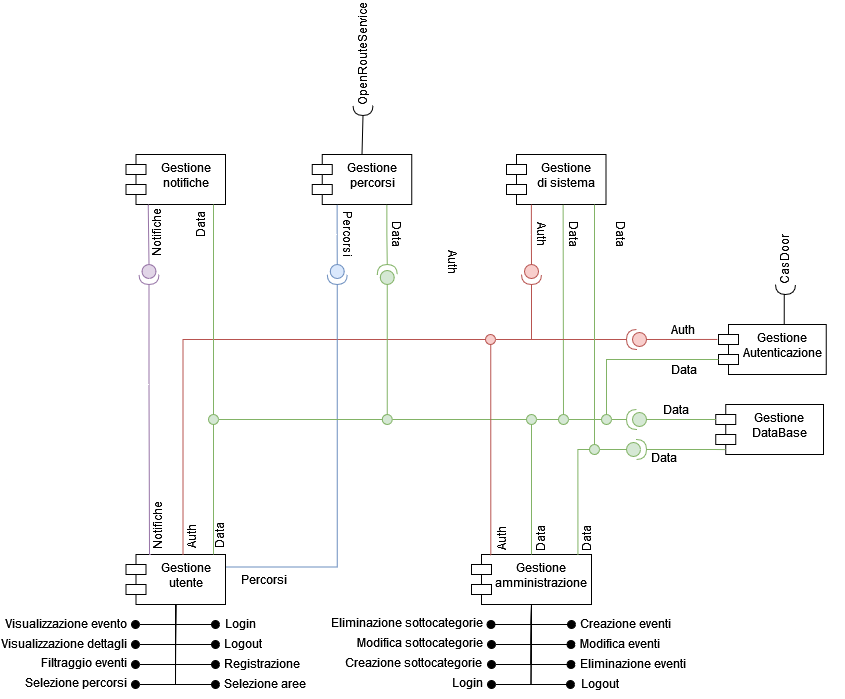
\includegraphics[width=1\textwidth]{Images/ComponentDiagram.png}
    \caption{Diagramma dei componenti}
    \label{fig:component-diagram}
\end{figure}

\end{document}